\documentclass[11pt]{article}

\usepackage{float}
\usepackage{hyperref}
\usepackage{graphicx}
% formatting
\usepackage{verbatim}
\usepackage{moreverb}
\usepackage{minted}
\usepackage{parskip}
\usepackage{amsmath}
\usepackage[listings]{tcolorbox}
\usepackage{enumerate}
\let\verbatiminput=\verbatimtabinput
\def\verbatimtabsize{4\relax}

\newcommand{\RepoRootPath}{fpga\_labs\_sp21}

\tcbset{
texexp/.style={colframe=black, colback=lightgray!15,
         coltitle=white,
         fonttitle=\small\sffamily\bfseries, fontupper=\small, fontlower=\small},
     example/.style 2 args={texexp,
title={Question \thetcbcounter: #1},label={#2}},
}

\newtcolorbox{texexp}[1]{texexp}
\newtcolorbox[auto counter]{texexptitled}[3][]{%
example={#2}{#3},#1}

\setlength{\topmargin}{-0.5in}
\setlength{\textheight}{9in}
\setlength{\oddsidemargin}{0in}
\setlength{\evensidemargin}{0in}
\setlength{\textwidth}{6.5in}

% Useful macros

\newcommand{\note}[1]{{\bf [ NOTE: #1 ]}}
\newcommand{\fixme}[1]{{\bf [ FIXME: #1 ]}}
\newcommand{\wunits}[2]{\mbox{#1\,#2}}
\newcommand{\um}{\mbox{$\mu$m}}
\newcommand{\xum}[1]{\wunits{#1}{\um}}
\newcommand{\by}[2]{\mbox{#1$\times$#2}}
\newcommand{\byby}[3]{\mbox{#1$\times$#2$\times$#3}}


\newenvironment{tightlist}
{\begin{itemize}
 \setlength{\parsep}{0pt}
 \setlength{\itemsep}{-2pt}}
{\end{itemize}}

\newenvironment{titledtightlist}[1]
{\noindent
 ~~\textbf{#1}
 \begin{itemize}
 \setlength{\parsep}{0pt}
 \setlength{\itemsep}{-2pt}}
{\end{itemize}}

% Change spacing before and after section headers

\makeatletter
\renewcommand{\section}
{\@startsection {section}{1}{0pt}
 {-2ex}
 {1ex}
 {\bfseries\Large}}
\makeatother

\makeatletter
\renewcommand{\subsection}
{\@startsection {subsection}{1}{0pt}
 {-1ex}
 {0.5ex}
 {\bfseries\normalsize}}
\makeatother

% Reduce likelihood of a single line at the top/bottom of page

\clubpenalty=2000
\widowpenalty=2000

% Other commands and parameters

\pagestyle{myheadings}
\setlength{\parindent}{0in}
\setlength{\parskip}{10pt}

% Commands for register format figures.

\newcommand{\instbit}[1]{\mbox{\scriptsize #1}}
\newcommand{\instbitrange}[2]{\instbit{#1} \hfill \instbit{#2}}
\newcommand{\itwos}{I\textsuperscript{2}S}

\begin{document}

\def\PYZsq{\textquotesingle}
\title{\vspace{-0.4in}\Large \bf EECS 151/251A FPGA Lab Spring 2021\\
Lab 6: UART\vspace{-0.1in}}

\author{Prof. John Wawrzynek \\
TAs: Sean Huang, Tan Nguyen \\ Department of Electrical Engineering and Computer Sciences\\
College of Engineering, University of California, Berkeley}
\date{}
\maketitle

\section{Before You Start This Lab}
You should run \verb|git pull| in \verb|fpga_labs_sp21| to get the latest files for this lab.

Copy the following files from previous labs to your working directory.
\begin{itemize}
  \item \verb|debouncer.v|
  \item \verb|synchronizer.v|
  \item \verb|edge_detector.v|
  \item \verb|fifo.v|
\end{itemize}

In this lab, we will implement a UART serial protocol for transmitting and receiving data over serial interface. We will use a Pmod USB-UART module connecting to the PYNQ-Z1 to interface with a host machine.

\section{UART Serial Device}
Recall the \href{http://inst.eecs.berkeley.edu/~eecs151/sp21/files/verilog/ready_valid_interface.pdf}{ready/valid handshake} that we learned in the previous lab to implement the FIFO module. The UART transmit and receive modules also use a handshake interface to communicate with other modules on the FPGA.

Both the UART’s receive and transmit modules will have their own separate set of ready/valid interfaces connected appropriately to external modules.

Please note that the serial line itself is not a ready/valid interface.
Rather, it is the modules you will work with in this lab (\verb|uart_transmitter| and \verb|uart_receiver|) that have the ready/valid handshake for interfacing with other modules on the FPGA.

The diagram below shows the entire setup:

\begin{figure}[H]
  \centerline{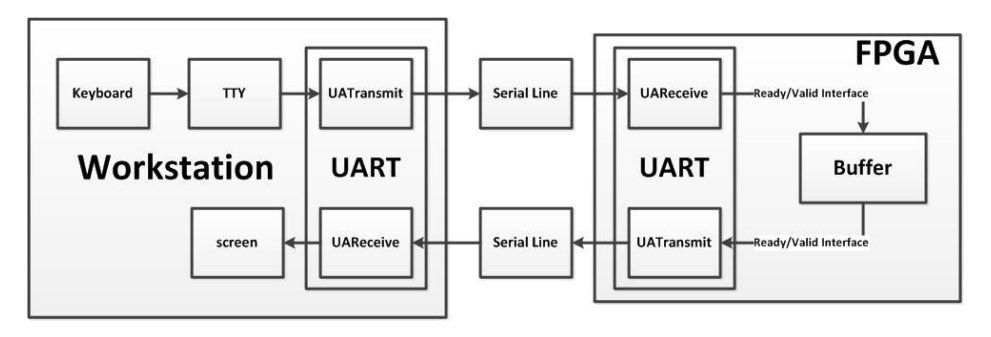
\includegraphics[width=6in]{figs/high_level_diagram.png}}
  \caption{High Level Diagram}
\end{figure}

In this lab, we'd like to ask you to implement the \verb|uart_transmitter| module. The \verb|uart_receiver| is provided to you.
In the process of testing your UART Transmitter, if you see some weird garbage symbols then the data is getting corrupted and something is likely wrong.
If you see this happening very infrequently, don't just hope that it won't happen while the TA is doing the checkoff; take the time now to figure out what is wrong.
UART bugs are a common source of headaches for groups during the first project checkpoint.

\subsection{PMOD USB-UART}
The PYNQ-Z1 does not have an RS-232 serial interface connected to the FPGA fabric.
So we'll be using the \href{https://store.digilentinc.com/pmod-usbuart-usb-to-uart-interface/}{Pmod USB-UART} extension module to add a UART interface to the Pynq.
Connect the PMOD module to the \textbf{top} row of the PMOD A port on the Pynq, and connect a USB cable from the USB-UART PMOD to your computer.

\textbf{Note:} Make sure that the power selection jumper on the Pmod USBUART is set to LCL3V3

\begin{figure}[H]
  \centerline{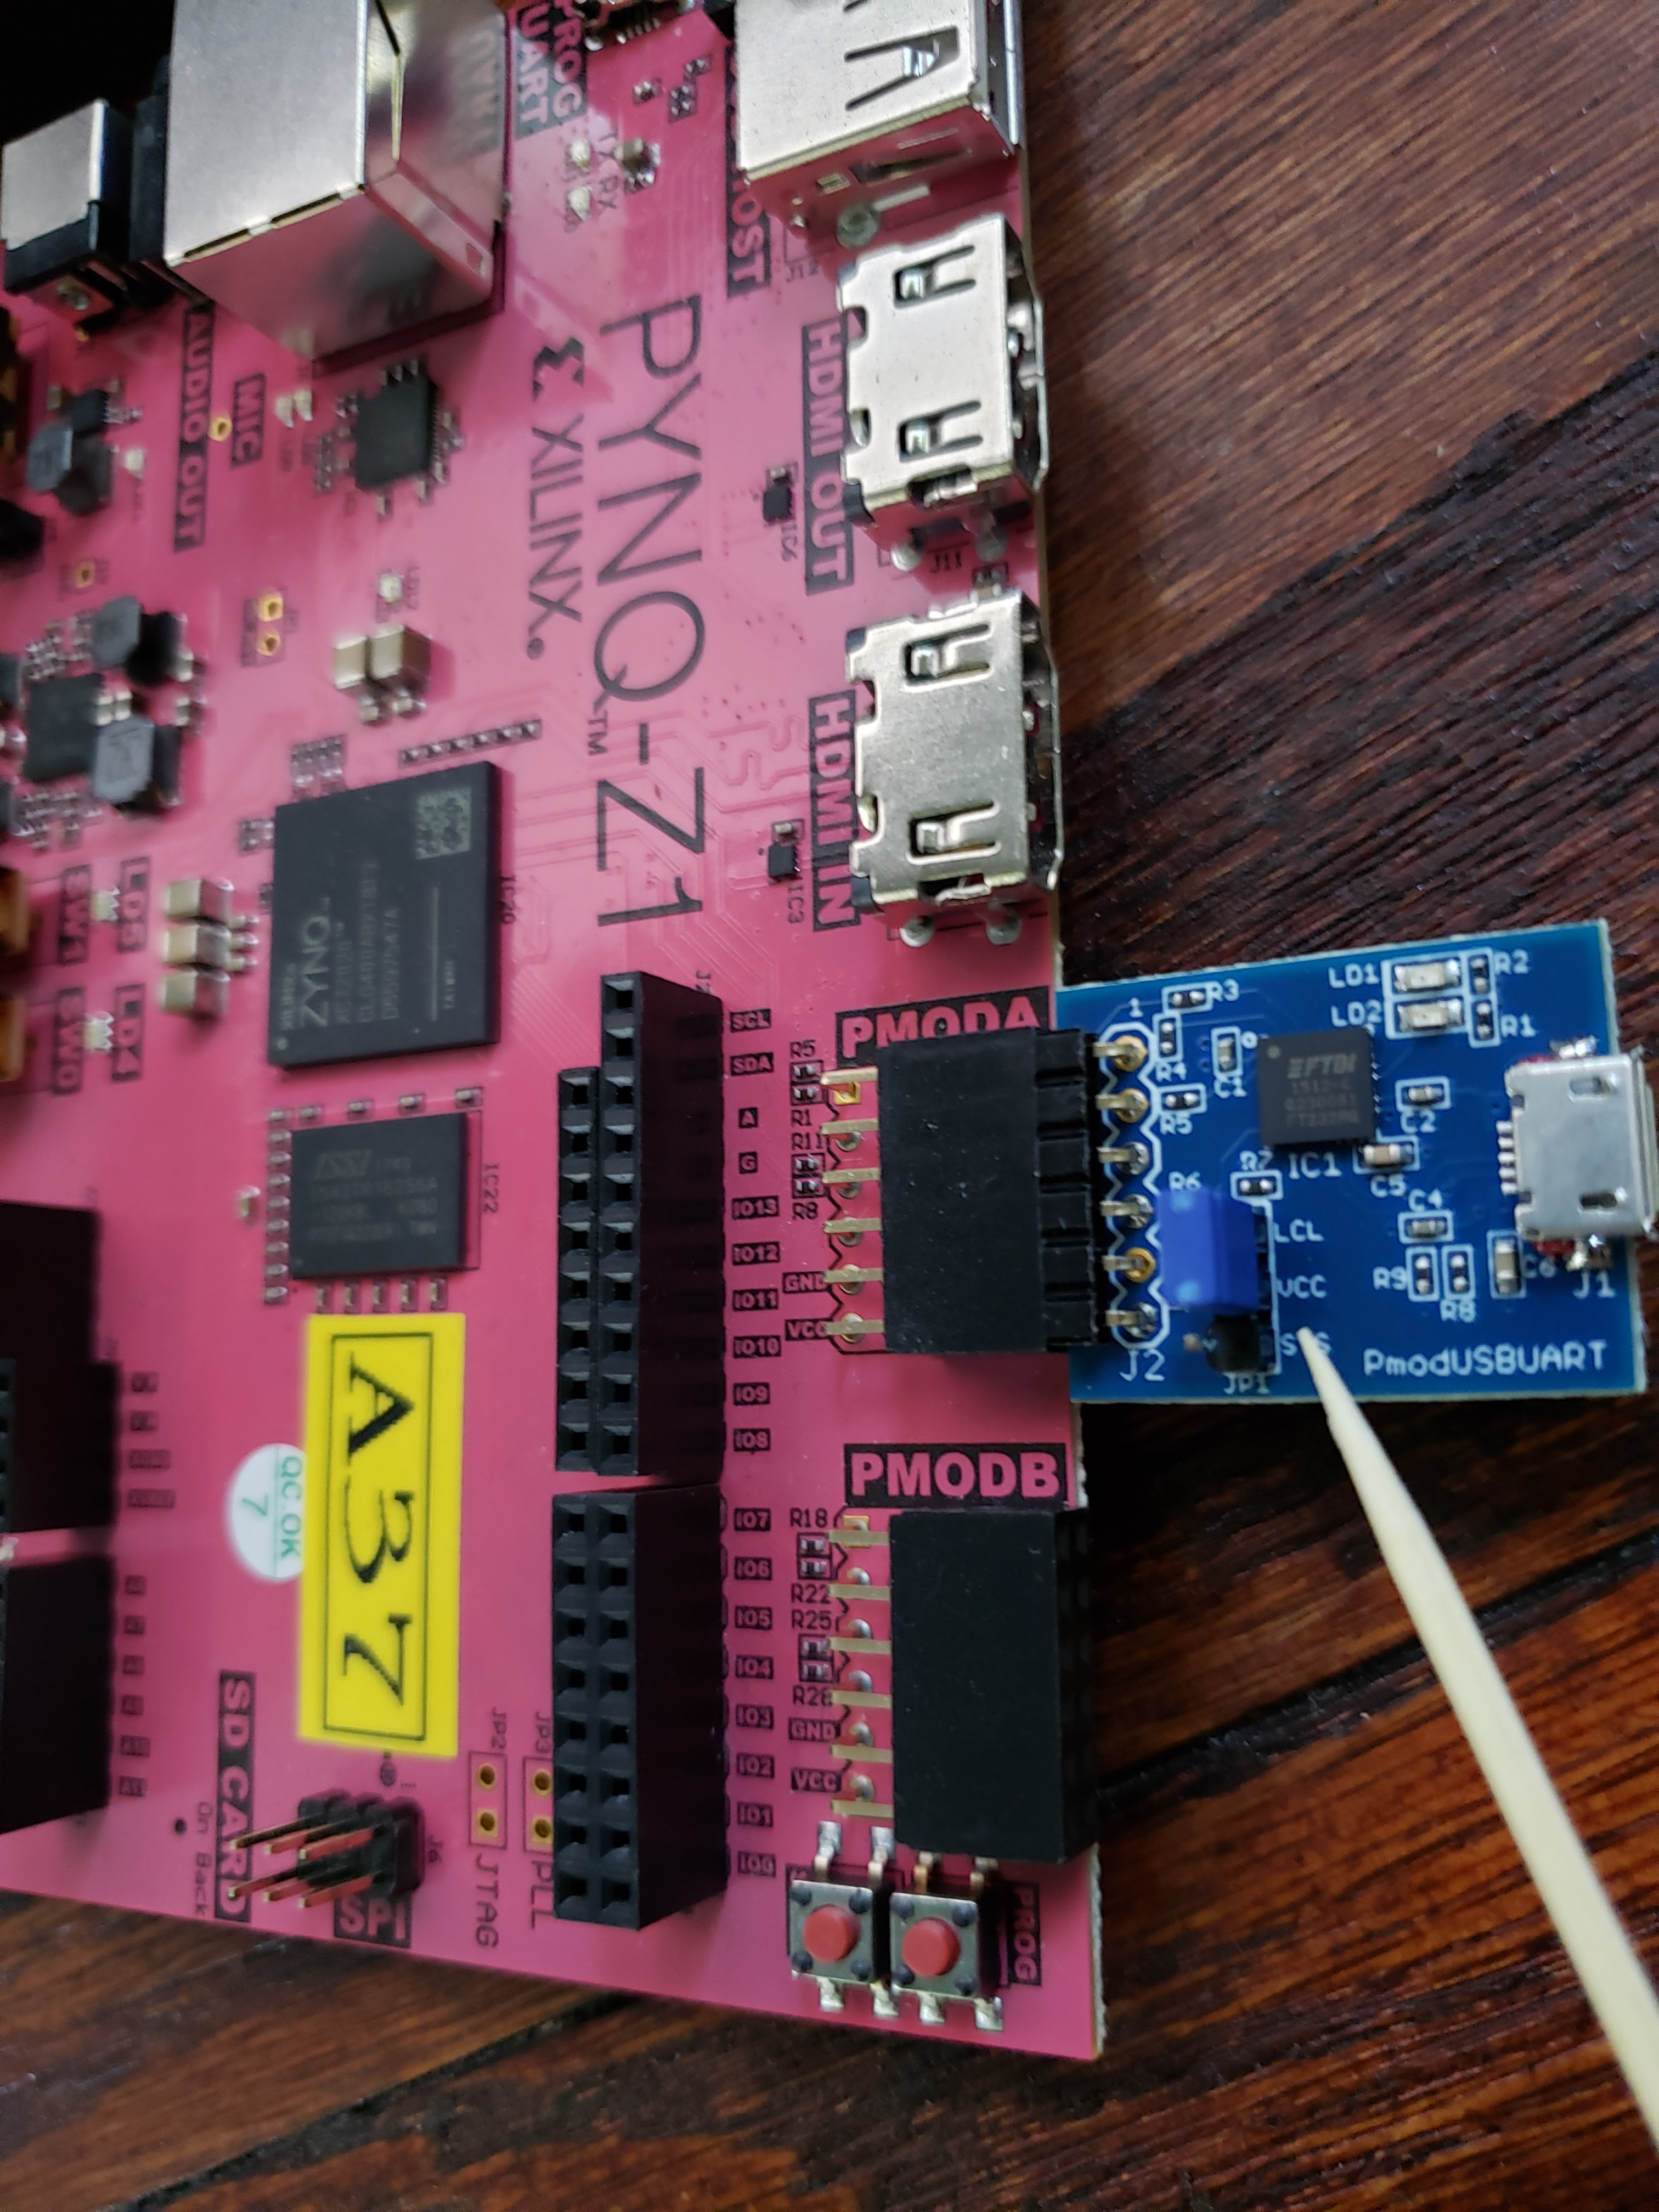
\includegraphics[width=2in]{figs/pmod_a.jpg}}
  \caption{PMOD USBUART plugged in w/ correct power jumper setting (blue).}
\end{figure}

\subsection{Framing}
On the \verb|PYNQ-Z1| board, the physical signaling aspects (such as voltage level) of the serial connection will be taken care of by off-FPGA devices.
From the FPGA's perspective, there are two signals, \verb|FPGA_SERIAL_RX| and \verb|FPGA_SERIAL_TX|, which correspond to the receive-side and transmit-side pins of the serial port.
The FPGA's job is to correctly frame characters going back and forth across the serial connection.
Figure 1 below shows a single character frame being transmitted.

\begin{figure}[H]
  \centerline{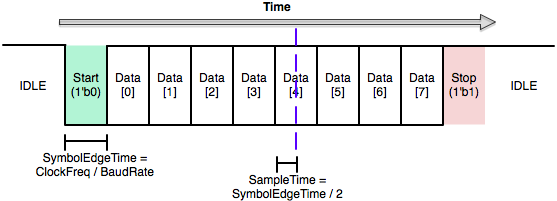
\includegraphics[width=6in]{figs/uart_frame.png}}
  \caption{UART Frame Structure}
\end{figure}

In the idle state the serial line is held high.
When the TX side is ready to send a character, it pulls the line low.
This is called the start bit.
Because UART is an asynchronous protocol, all timing within the frame is relative to when the start bit is first sent (or detected, on the receive side).

The frame is divided up in to 10 uniformly sized bits: the start bit, 8 data bits, and then the stop bit.
The width of a bit in cycles of the system clock is given by the system clock frequency divided by the baudrate.
The baudrate is the number of bits sent per second; in this lab the baudrate will be 115200.
Notice that both sides must agree on a baudrate for this scheme to be feasible.

\subsection{UART Transmitter}

\begin{center}
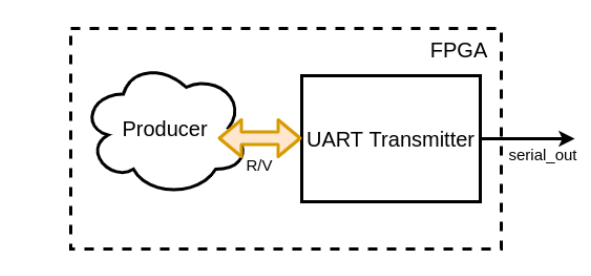
\includegraphics[width=0.4\textwidth]{figs/uart_tx.png}
\end{center}

The UART Transmitter receives a character from a producer block on FPGA via Ready/Valid interface. Once we have a character that we want to send out (i.e., once Valid goes HIGH, and the transmitter is ready), transmitting it is simply a matter of shifting each bit of the read character, plus the start and stop bits, out of a shift register on to the serial line.

Remember, the serial baudrate is much slower than the system clock, so we must wait $SymbolEdgeTime = \frac{ClockFreq}{BaudRate}$ cycles between changing the character we're putting on the serial line.
After we have shifted all 10 bits out of the shift register, we are done unless we have to send another frame immediately after. The transmitter should not be ready when it is in a middle of sending a frame.

\textbf{Your task} is to complete the implementation of UART Transmitter in the file \verb|lab5/src/uart_transmitter.v|.

\subsubsection{Testing}

The \verb|z1top_uart_tx| module stores a text data locally in the block RAMs. The role of the UART Transmitter is to send all the bytes from the text data to your workstation over the serial interface. You should be able to see the text on your serial terminal after loading the bitstream.

\begin{center}
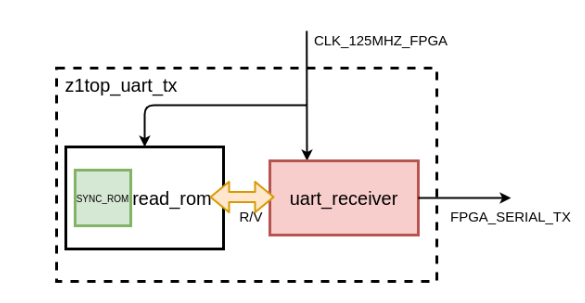
\includegraphics[width=0.4\textwidth]{figs/z1top_uart_tx.png}
\end{center}

Similar to the previous exercise, you will need to use the following commands to build, implement, and test your project with the UART Transmitter module. The provided testbench tests if your UART Transmitter can read multiple charactes successively and transmit them via the serial line.

\begin{minted}{bash}

# Build Vivado project z1top_uart_tx_proj
make build-project proj=z1top_uart_tx

# Simulate with sim/uart_transmitter_tb.v
make sim proj=z1top_uart_tx tb=uart_transmitter_tb

# Generate bitstream
make write-bitstream proj=z1top_uart_tx

# Program the FPGA
make program-fpga bs=bitstream_files/z1top_uart_tx.bit
\end{minted}

If you are more comfortable with the GUI mode, you can open the Vivado project right after the \texttt{make build-project} command. (or create a project and add files manually.)

\subsubsection{Terminal Program}
On your workstation or VM (that connects to the FPGA), run:

\begin{minted}{bash}
# If you see the message "Screen is terminating", try running the command with sudo
screen $SERIALTTY 115200
\end{minted}

This tells \verb|screen|, a serial terminal, to open up the serial device with a baud rate of 115200 (you might have to run this with \verb|sudo| on your laptop). If \verb|$SERIALTTY| is not defined on your laptop, look for the name of the device file that the Serial Device is attached to, e.g. \verb|/dev/ttyUSB0| using \texttt{dmesg}. See the Appendix for more information.

To close \verb|screen|, type \verb|Ctrl-a| then \verb|Shift-k| and answer \verb|y| to the confirmation prompt.
If you are using a lab machine and you don't close the screen program properly, other students won't be able to access the serial port on your workstation.

If you try opening \verb|screen| and it terminates after a few seconds with an error saying ``Sorry, can't find a PTY'' or ``Device is busy'', execute the command \verb|killscreen| which will kill all open screen sessions that other students may have left open.
Then run \verb|screen| again.

Use \verb|screen -r| to re-attach to a non-terminated screen session. You can also reboot the computer to clear all active \verb|screen| sessions.

After the FPGA is programmed, turn on \verb|SWITCHES[1]|. The text will appear on the serial terminal. Press \verb|BUTTONS[0]| to reset, and the text will reappear. You can also use the \verb|BUTTONS| and \verb|SWITCHES[0]| to provide input to the UART Transmitter. Read the code \verb|lab5/src/z1top_uart_tx.v| to see what should be expected.

\subsection{UART Receiver}

\begin{center}
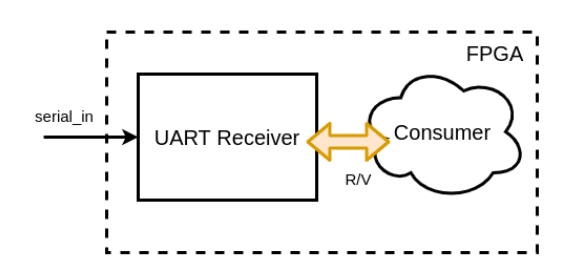
\includegraphics[width=0.4\textwidth]{figs/uart_rx.png}
\end{center}

The receive side of the serial device is essentially just a shift register to shift bits from the serial line.
However, care must be taken into determining when to shift bits in.
If we attempt to sample the serial signal directly on the edge between two symbols, we are likely to sample on the wrong side of the edge and get the wrong value for that bit.
One solution is to wait halfway into a cycle (until \verb|SampleTime| on the diagram) before reading a bit in to the shift register.

In addition, the UART Receiver module sends the received character to a consumer block on FPGA via the Handshake interface. Therefore, once we have received a full character over the serial port, the Valid signal should go HIGH until the Ready signal goes HIGH, after which the Valid signal will be driven LOW until we receive another character.

You do not need to implement the UART Receiver as it is provided to you.

\subsection{UART Echo -- Putting It All Together}

In this section, you will put both the UART Receiver and Transmitter together, and attempt to communicate with a serial terminal on your workstation. That means you will be able to provide input to the FPGA using the keyboard of your workstation instead of just buttons and switches!

\textbf{Your task} is to complete the implementation of the UART module in the file \verb|lab5/src/uart.v|. The UART module receives a character from the input serial line, and performs case inversion if it is a letter (lowercase to uppercase and vice versa), and sends the result to the output serial line. Once you're done with the implementation, use the following commands to build, simulate, and generate bitstream for your project.

\begin{minted}{bash}

# Build Vivado project z1top_uart_echo_proj
make build-project proj=z1top_uart_echo

# Simulate with the testbench echo_tb
make sim proj=z1top_uart_echo tb=echo_tb

# Generate bitstream
make write-bitstream proj=z1top_uart_echo

# Program the FPGA
make program-fpga bs=bitstream_files/z1top_uart_echo.bit
\end{minted}

Now, open \verb|screen| as similar to previous sections. Try hitting your keyboard really hard and fast and see if you can get all the characters echoed back (with case inversion for letters). Let's try an even harder test. We will run a Python script to read a text file on your local workstation, send the file to the PYNQ via the serial line, and observe the content of the file on a serial terminal.

\begin{minted}{bash}
# Before you run the following command, make sure that you install the required
# Python packages on your workstation. If you are using the lab machines,
# you do not need to worry about this.
# The pyserial package is likely needed:
sudo pip3 install pyserial

# This command will send a text file (z1top_uart_echo.v in this example) to the FPGA
# over the serial line.
/usr/bin/python3 scripts/echo.py src/z1top_uart_echo.v

# You can also try sending a larger file to stress the UART pipeline
\end{minted}

After the script prompts for user input, open \verb|screen| as usual in a separate terminal before hitting \texttt{Enter}. If everything goes well, you should see the text content shown in the serial terminal. If you see the text corrupted, you can try increasing the time interval between sending successive characters in the script. Is there another solution for this that you can implement in \verb|lab5/src/uart.v|?

Ultimately, the motivation here is to ensure that you can send the external data to your FPGA over the serial line without any corruption. In the final project, the external data is the program or command that you would like to execute on the processor that you implement on the PYNQ. The UART pipeline provides a means to communicate with your processor by loading and running different programs as well as observing the results from your own workstation in a more systematic and pragmatic manner than relying on the buttons, switches, and LEDs on the PYNQ as we did in previous labs.

If everything is working well, good work! Your UART Transmitter is now thoroughly tested.

\subsection{Questions}\label{sec:Q1}
\begin{enumerate}
\item How did you design your UART Transmitter? Please draw some block diagram of your design, and if applicable, a state transition diagram if you use FSM to design the control logic of your UART Transmitter module.
\item Regarding the \verb|lab5/src/uart.v| implementation, what could be an issue if we try sending characters to the UART pipeline at a very high speed (e.g., by using the script as above)? What can you do to fix the issue?
\end{enumerate}

\section{Drawing Triangle}

This section intends to walk you through the timing closure problem in FPGA design. Designing a hardware block isn't just a matter of getting correct answers or functionality; we also use the QoR (Quality-of-Result) as metrics of goodness to evaluate it. Typically, the QoR concerns with the cost (area) and the performance (number of cycles $\times$ clock frequency). Timing closure is a process of optimizing your circuit to meet a target frequency. So far, we have been dealing with small circuit designs that utilize very few LUTs or FFs. The tool does not have any challenges in placing and routing your circuits to meet the target timing (typically 125 MHz). In this section, we will work with a moderate-size circuit that involves lots of wide-width arithmetic operations, such as addition, subtraction, comparators, and multiplication of 32-bit signals. We will optimize the circuit to satisfy a target clock frequency. To do so, you should identify the critical path in your design. The critical path is the path between two registers (or flip-flops) that has the longest propagation delay. One simple, yet powerful technique of improving the timing of a digital circuit is pipelining: we essentially place some registers on the critical path to break it into shorter paths. However, this will change the \textit{semantics} of your implementation, since now the cut path would require two clock cycles to complete instead of one. In addition, you must make sure that other paths parallel with that path are also properly registered (timed) to ensure the behavioral correctness of your pipelined circuit. Pipelining presents a design tradeoff in terms of frequency versus area (number of registers) and number of cycles. Another technique is re-timing, where one moves an existing register on a path to balance the delays of the subpaths to achieve better timing.

Let's look at a concrete example.

\begin{center}
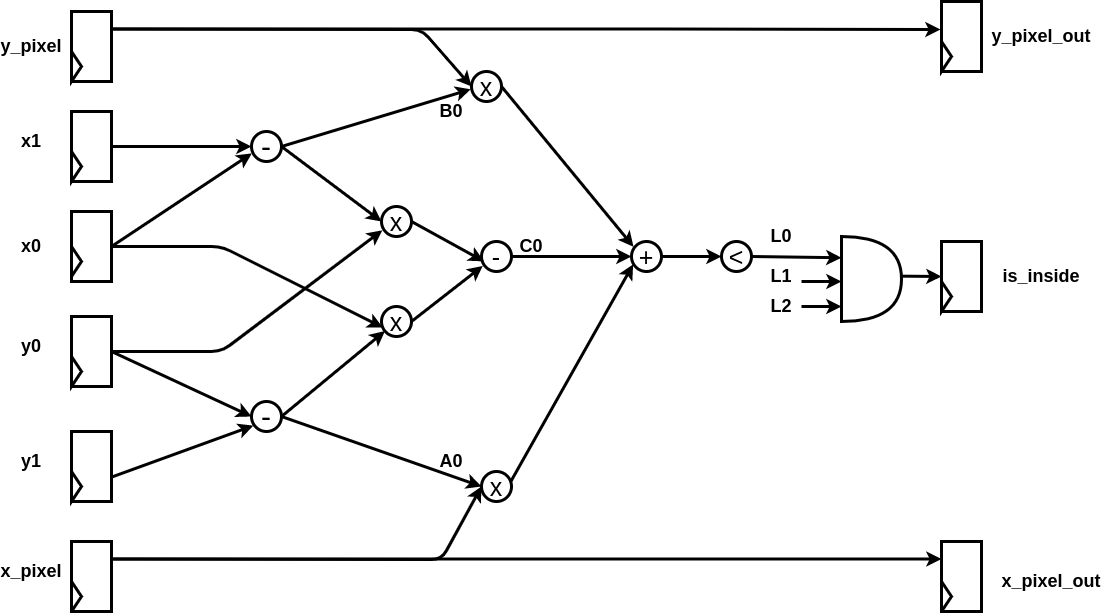
\includegraphics[width=0.6\textwidth]{figs/inside_test.png}
\end{center}

This circuit (partially shown for brevity) tests if a pixel is inside a triangle. Suppose we want to draw a triangle given the pixel coordinates of the three vertices. At every pixel of an image, we would like to test if the pixel is inside the triangle. One way of doing so is to test the relative position of the pixel to the lines formed by each pair of the three vertices. If the pixel is on the same side for all three lines, it is inside the triangle, and we assign the pixel with a color. You can read about it more from the \href{https://cs184.eecs.berkeley.edu/sp19/lecture/2/rasterization}{Computer Graphics CS184 lecture}. However, you really don't need to know the details of the math. We have provided a working \verb|inside_test| circuit design in the file \verb|lab5/src/inside_test.v|. Your task is to figure out where to put pipeline stage(s) to meet the required clock frequency.

In addition, you need to modify the file \verb|lab5/src/draw_triangle.v| to implement proper video signals as similar to the \verb|display_controller.v|, but you should use \verb|pixel_x_out| and \verb|pixel_y_out| to drive the video signals instead. This module is similar to the \verb|display_controller.v|, except that now we stream a graphical object drawn by our circuit in real time instead of a static image.

The file \verb|lab5/src/z1top_draw_triangle.v| is the top-level module that interfaces with Digilent video IP to draw a triangle to a monitor. It also instantiates the UART modules so that you can move the triangle using the keyboard of your workstation.
You only need to modify \verb|PIXEL_CLK_PERIOD| parameter to change the target pixel clock period of your system. For this exercise, we will configure video output with a resolution of 1280 $\times$ 720 @60Hz. That would require a pixel clock of 74.25 MHz. You are expected to pipeline the \verb|inside_test| module to meet the target clock period of \textbf{14 ns}. To build and test your project, use the following commands.

\begin{minted}{bash}

# Build Vivado project z1top_draw_triangle_proj
make build-project proj=z1top_draw_triangle

# Simulate with sim/inside_test_tb.v
make sim proj=z1top_draw_triangle tb=inside_test_tb

# Generate bitstream
# Before generating bitstream, make sure that you have implemented the video timing signals
# properly in src/draw_triangle.v
make write-bitstream proj=z1top_draw_triangle

# The timing report can be found at
# z1top_draw_triangle_proj/z1top_draw_triangle_proj.runs/\
# impl_1/z1top_draw_triangle_bd_wrapper_timing_summary.rpt

# Program the FPGA
make program-fpga bs=bitstream_files/z1top_draw_triangle.bit
\end{minted}

Every time you make change to the \verb|inside_test| module, you should run a simulation to ensure that the functionality is still correct. A testbench has been provided for this purpose: \verb|lab5/sim/inside_test_tb.v|. Once you pass the simulation, generate the bitstream and check the timing report to see if your design meets timing. A negative slack means a path in your design fails to meet the target clock period, and you should fix it. Look at the \textit{VIOLATED} path(s) in the report, try to make sense of how that path corresponds to your Verilog code, and the delay at each primitives on which the signal traverses that path, this should give you a hint of where to place your register(s) to cut the path. There are two sources of delay: logic delay and net delay. The former concerns with how you design your circuit in Verilog (at the schematic level), while the latter depends largely on how the tool places and routes your design on a target device. We can also rely on the tool to visualize the critical path post Implementation. Below is one example that shows a path failed to meet 19ns. You will need to click \textit{Open Implemented Design} after the implementation to see this. You can also switch to the Schematic view to see what the primitives are on the path.

\begin{center}
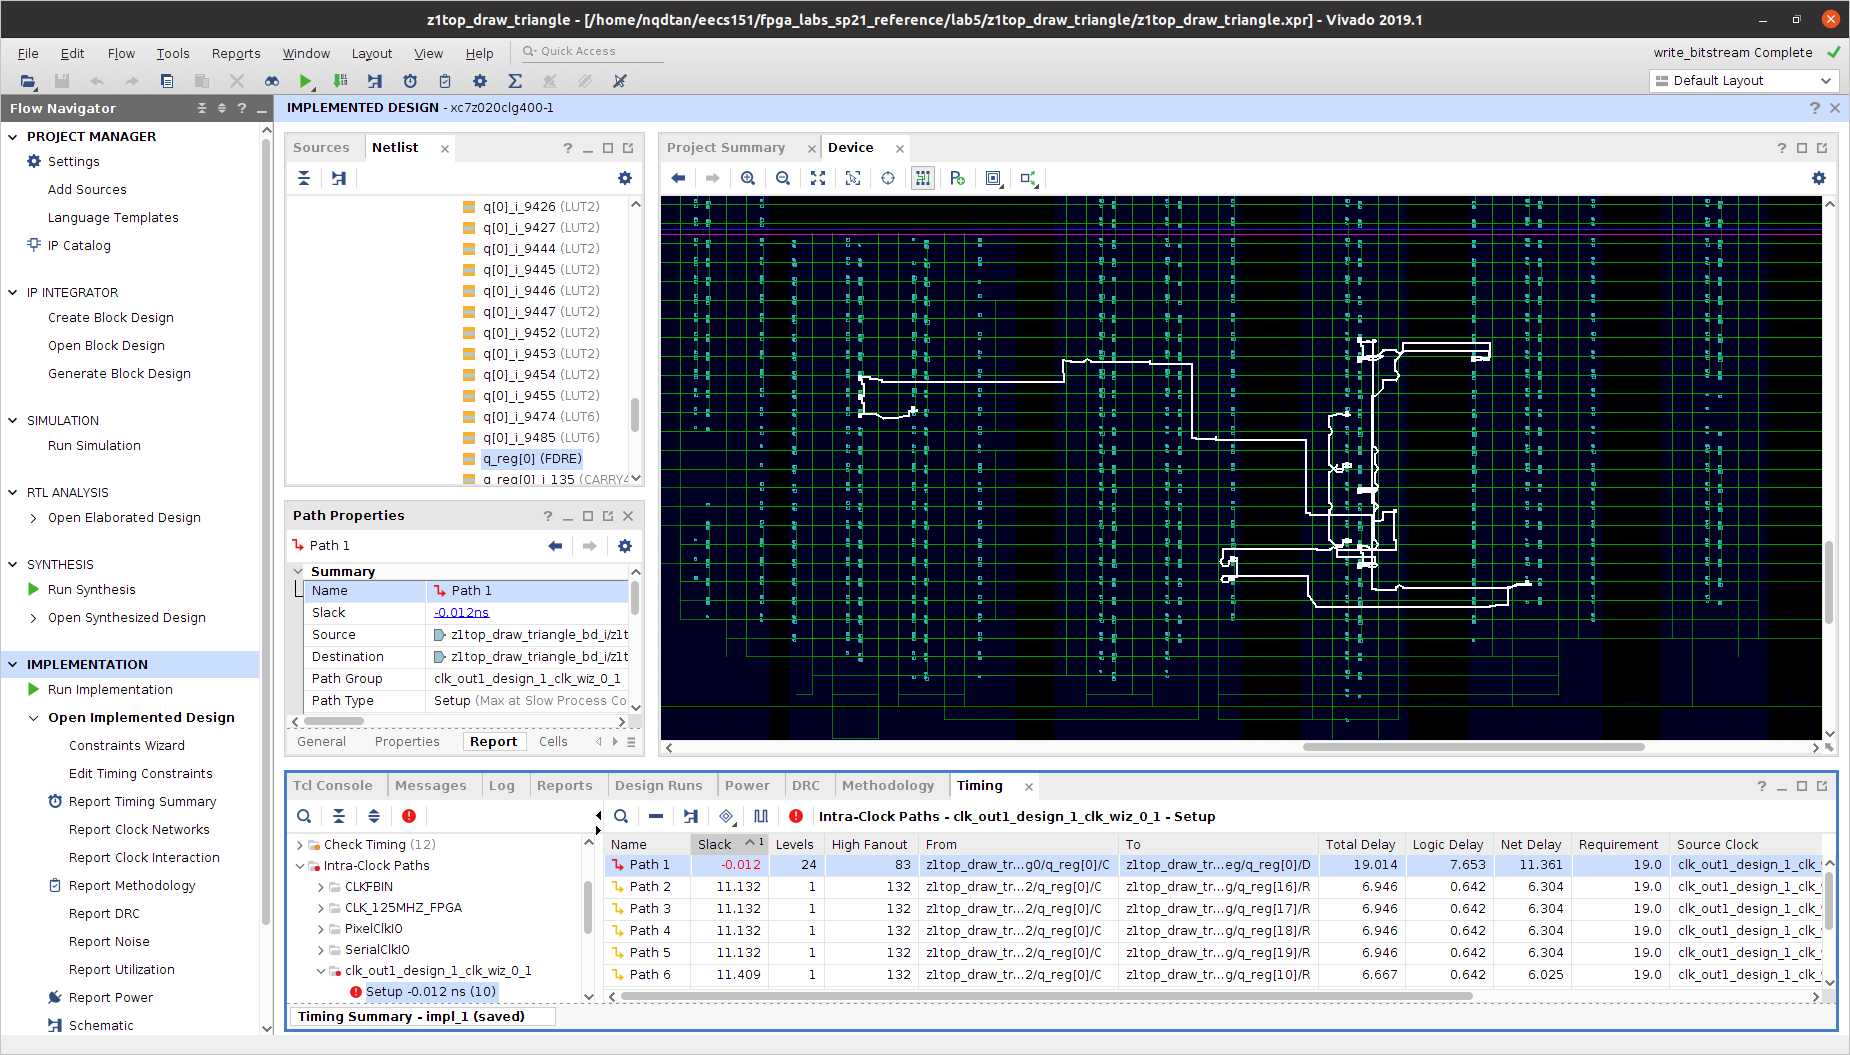
\includegraphics[width=0.8\textwidth]{figs/critical_path_vivado.png}
\end{center}

Since your design eventually boils down to FPGA primitives such as LUTs, FF, carry chains, etc., sometimes it is difficult to tell exactly how the paths in the report are relevant to your Verilog source code. When inspecting a timing report to find a critical path in your design, one tip is to pay attention to the \textit{Source} and the \textit{Destination} of a path that has the most negative slack. This should help you trace the path back to your code. One feedback from previous semester regarding the use the \texttt{REGISTER*} modules instead of sequential always blocks is it helps to locate the paths fairly easily due to the hierarchy of module instantiations. In some cases, the tool might also flatten the design in order to merge some logic across module boundaries for further optimization, and as the original signals' names might be changed during that process, it would be harder to trace the paths back to the source.

Nonetheless, you can make some educated guess of the delays of your paths based on the high-level dataflow graph of your circuit, as shown in the \textit{inside\_test} figure above. For instance, the delay on a path with a multiplier followed by a subtractor and a comparator probably takes longer than a path with only an adder. Remember that FPGA is a spatial computing device, everything you write comes with a cost (area or delay). Think carefully of which operators should you use. For example, if you want to scale a signal down, you will need to think twice before deciding to use a divide operator; a right shift is much better in terms of hardware cost and is more FPGA-friendly. Depending on the quality of your FPGA board, a slightly negative-slack implementation can still work sometimes, but don't take it for granted. You should develop a practice of checking the timing report every time you finish implementation, and then fix any timing issues you may discover in your design.

\subsection{Questions}\label{sec:Q2}
\begin{enumerate}
\item How many pipeline stages did you insert to your design to meet 14ns? And where did you put them? You can draw the stages on the circuit figure above.
\item How do you think the wide-width arithmetic operators, such as adders, comparators, are implemented on the FPGA? You don't have to work to the details; just need to provide a general sense of how the primitives are connected (among the slices) to form such operators. The Schematic might be helpful.
\item Remove the "use\_dsp = no" attribute in \verb|lab5/src/inside_test.v|, and run the implementation to obtain the area report. Compare the area utilizations between the two (unpipelined) designs in terms of LUTs, FFs, DSPs, and CARRY4.
\item Can you mention a few advantages and disadvantages of using the DSP blocks (it helps to be aware of where they are on the device, and their layout in comparison to the slices)?
\item One could instantiate multiple drawing engines to draw more triangles in parallel. How many triangles can we draw on the PYNQ-Z1 if we use LUTs (and CARRY4) only? How many triangles can we draw if we can also utilize the DSP blocks?
\end{enumerate}

%\newpage
\section{Lab Deliverables}
\subsection{Lab Checkoff (due: 11.00AM, Mar 10th, 2021)}
To checkoff for this lab, have these things ready to show the TA:
\begin{enumerate}
  \item Demonstrate that your UART Transmitter is working properly by showing demos with the top-level modules \verb|z1top_uart_tx| and \verb|z1top_uart_echo|.
  \item Demonstrate that your \verb|z1top_draw_triangle| module meets a pixel clock period of 14 ns.
\end{enumerate}

\subsection{Lab Report  (due: 11.59PM, Mar 10th, 2021)}\label{sec:labreport}
\begin{enumerate}
  \item Your answers to the questions in sections \ref{sec:Q1} and \ref{sec:Q2}.
\end{enumerate}

\appendix
\section{Personal Laptop Instructions}

\subsubsection{Linux/OSX}
After plugging in the USB cable, run \verb|dmesg| and observe the output:
\begin{minted}{text}
[7444636.941491] ftdi_sio 1-2:1.0: FTDI USB Serial Device converter detected
[7444636.941621] usb 1-2: Detected FT232RL
[7444636.942062] usb 1-2: FTDI USB Serial Device converter now attached to ttyUSB0
\end{minted}

Then connect using \verb|sudo screen /dev/ttyUSB0 115200|

\subsubsection{Windows}
After plugging in the USB cable, you may be prompted to install the FTDI drivers, so do that.
Follow the \href{https://xilinx-wiki.atlassian.net/wiki/spaces/A/pages/18842446/Setup+a+Serial+Console}{steps from here} to use PuTTY to connect to the UART.

%\newpage
\section*{Ackowlegement}
This lab is the result of the work of many EECS151/251 GSIs over the years including:
\begin{itemize}
\item Sp12: James Parker, Daiwei Li, Shaoyi Cheng
\item Sp13: Shaoyi Cheng, Vincent Lee
\item Fa14: Simon Scott, Ian Juch
\item Fa15: James Martin
\item Fa16: Vighnesh Iyer
\item Fa17: George Alexandrov, Vighnesh Iyer, Nathan Narevsky
\item Sp18: Arya Reais-Parsi, Taehwan Kim
\item Fa18: Ali Moin, George Alexandrov, Andy Zhou
\item Sp19: Christopher Yarp, Arya Reais-Parsi
\item Fa19: Cem Yalcin, Rebekah Zhao, Ryan Kaveh, Vighnesh Iyer
\item Sp20: Tan Nguyen
\item Fa20: Charles Hong, Kareem Ahmad, Zhenghan Lin

\end{itemize}

\end{document}
